\documentclass[conference]{IEEEtran}
\IEEEoverridecommandlockouts
% The preceding line is only needed to identify funding in the first footnote. If that is unneeded, please comment it out.
\usepackage{cite}
\usepackage{amsmath,amssymb,amsfonts}
\usepackage{algorithmic}
\usepackage{graphicx}
\usepackage{textcomp}
\usepackage{xcolor}
\usepackage{hyperref}
\usepackage{float}
\usepackage{ngerman}
\def\BibTeX{{\rm B\kern-.05em{\sc i\kern-.025em b}\kern-.08em
    T\kern-.1667em\lower.7ex\hbox{E}\kern-.125emX}}
\begin{document}

\title{Dokumentation der Softwarearchitektur des Projekts Explosion Guy}


% Authoren	
\author{
	\IEEEauthorblockN{Bösl Florian}
	\IEEEauthorblockA{
		\textit{f.boesl@oth-aw.de}\\
	}
	\and

	\IEEEauthorblockN{Kohl Helge}
	\IEEEauthorblockA{
		\textit{h.kohl@oth-aw.de}\\
	}
	\and

	\IEEEauthorblockN{Chernysheva Anastasia}
	\IEEEauthorblockA{
		\textit{a.chernysheva@oth-aw.de}\\
	}
	\and

	\IEEEauthorblockN{Korinth Patrice}
	\IEEEauthorblockA{
		\textit{p.korinth@oth-aw.de}\\
	}
	\and

	\IEEEauthorblockN{Porsch Philipp}
	\IEEEauthorblockA{
		\textit{p.porsch@oth-aw.de}\\
	}
}

\maketitle

\begin{abstract}
In diesem technischem Report wird die Softwarearchitektur des Projekts 
Explosion Guy vorgestellt. Das Projekt wurde im Rahmen der Vorlesung Big Data und Cloud-basiertes Computing implementiert. Ziel der Implementierung ist es, 
das allgemein bekannte Spiel \glqq Bomberman\grqq{} zu adaptieren und es mithilfe einer Cloud-Infrastruktur online spielbar zu machen.\\
\end{abstract}

\begin{IEEEkeywords}
 Webdesign, Matchmaking, Cloud Infrastructure
\end{IEEEkeywords}

\section{Introduction}
Bei der Applikation Explosion Guy geht es darum, das Spiel \glqq Bomberman\grqq{} zu adaptieren. Dabei werden dem Spieler mithilfe eines graphischen Web-Interfaces, basierend auf Phaser\cite{phaser}, anschauliche Informationen über den Verlauf des Spiels mitgeteilt. Das Interface dient auch dazu, die Eingaben des Spielers an das Backend weiterzureichen. Im Backend werden die Informationen aller Spieler verarbeitet und so ein Online-Spielerlebnis erzeugt.

\section{Architektur Allgemein}
\begin{figure*}
    \centering
    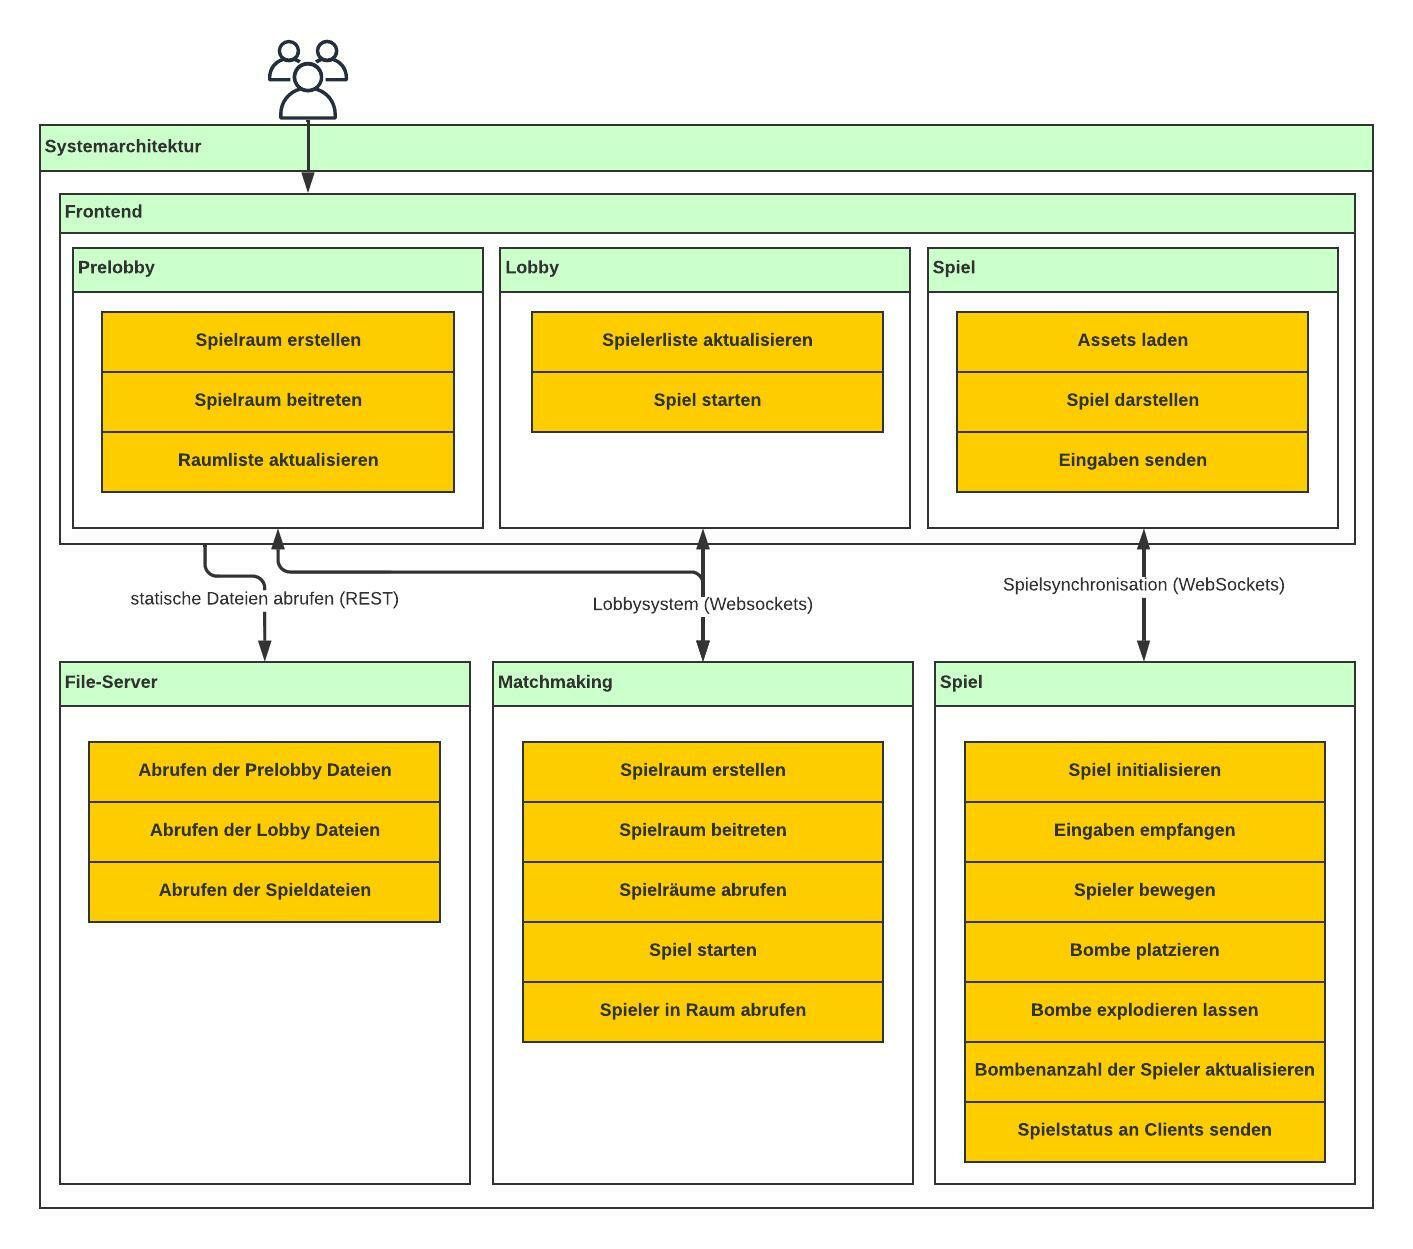
\includegraphics[width=\textwidth]{architecture.jpeg}
    \caption{Übersicht Gesamtsystem}
\end{figure*}
Als Architektur wird ein Ansatz verfolgt, der sich an einer Client-Server Kommunikation, ähnlich wie in anderen Onlinespielen, orientiert.
Dadurch wird eine abgeschlossene Logik von Front- und Backendkomponenten erreicht, die jeweils
von einem Subteam entwickelt wird. Diese Einheiten werden jeweils als isolierte Applikation gekapselt. Während das Backend als Anwendung innerhalb der Containervisualisierung Docker\cite{docker} betrieben wird, wird das Frontend als allgemeine Webapplikation ausgeliefert. Durch eine zentrale Konfigurationsdatei des Containers kann dieser einfach zwischen den Teammitgliedern ausgetauscht und ausgeführt werden. Damit wird eine hohe Portabilität gewährleistet.
Die Kommunikation der Teilsysteme wird durch Websockets\cite{socketio} angeboten. Der Informationsaustausch über Websockets ermöglicht es, durch die identitätsbasierten Verbindungen die Kommunikation zwischen den Spielern und der zugehörigen Partei im Backend effizient zu gestalten.
Dadurch wird es möglich ein Echtzeiterlebnis mit zusätzlicher Überwachung aus dem Backend zu realisieren.
Durch die Einbettung der verschiedenen Bestandteile in einen Cloud-Service ist es jederzeit möglich, ein neues Spiel zu starten, oder einem vorhandenen Spiel beizutreten, da durch die nahezu unbegrenzten Ressourcen des Cloud-Services auf Anfrage neue Spielserver erstellt und verwaltet werden können.

\section{Frontend: Spielinterface}
% TODO:
Mithilfe des Web-Frameworks Phaser\cite{phaser} ist es möglich, ein graphisch ansprechendes Interface für das Spiel zu erstellen. Dabei werden nicht nur die Ausgangsinformationen in Form von Veränderungen des Spielfeldes für den Spieler bereitgestellt, sondern auch die Eingaben an das System vom Spieler erfasst. Diese Eingaben leitet das Frontend an das Backend weiter, von wo aus sie dann weiter verarbeitet werden können. Um ein möglichst flüssiges und ruckelfreies Spielerlebnis zu erzeugen, wurde das Frontend auch mit Teilen der Spiellogik ausgestattet. So können beispielsweise alle Bewegungen direkt nach Drücken der entsprechenden Eingabe ausgeführt werden, ohne die Antwort des Backends abzuwarten, um Verzögerungen zu vermeiden. Sollte der Server nach Kontrolle einen ungültigen Spielzug feststellen, so wird der Zug zurückgesetzt. Dies erfüllt neben der Aufwertung des Gameplays auch eine kleine Anti-Cheating-Rolle.
\\
\\
Um die Funktionen des Frontends besser verwalten zu können, wurde es in folgende Klassen aufgeteilt:

\begin{itemize}
    \item \textbf{Main}
    Main stellt die Hauptverwaltungsklasse dar. In ihr werden die Objekte aus dem Backend übermittelt, wie etwa gamedata. Dies wird genutzt, um eine dynamische Erstellung des Spielfelds in der Create-Methode zu erlauben. Die Objekte bieten etwa Informationen über Größe und Breite des Spielfelds sowie die unterschiedlichen Blöcke auf dem Spielfeld, die die sogenannten 'Tiles' darstellen. Mit Hilfe der Informationen werden im Frontend Layer generiert, auf die anschließend mittels der addPropToLayer-Funktion die Blöcke erstellt werden mit Eigenschaften wie der Kollision. In der Update-Methode werden bei jedem Frame-Update die Inputs des Spielers überprüft. Die Bewegungsanweisungen werden über die entsprechende Pfeiltaste getriggert. Die Anweisungen werden zuerst an das Backend geschickt, jedoch auch sofort im Frontend verarbeitet, sodass es zu einer Überprüfung der Tiles kommt, um Lagging zuvorzukommen und ein Glitchen durch Wände zu verhindern. Zusätzlich werden passende Animationen abgespielt, die bei Nichteingabe pausiert werden. Die Informationen über gesetzte Bomben, Spielerpositionen sowie die isAlive-Abfrage werden aus dem Backend bezogen und auch hier verarbeitet.
    \smallskip
    \item \textbf{Player} 
	In der Playerklasse werden über den Konstruktor zunächst wichtige Informationen wie die ID, den isAlive-Status sowie die Position festgelegt. Die bomboutLines stellen Sprites da, die für die momentane Anzahl der Bomben des Player stehen. Die Kill-Methode deaktiviert den Spieler wenn dieser von einer Bombe getroffen wird und setzt den visible-Status des Sprites auf false.
    \smallskip
    \item \textbf{Explosion}
    Die Explosion-Klasse ist für Visualisierung der Bombenexplosion zuständig und spielt beim Explodieren eine Animation ab und lässt per Kamera-Shake das Spielfeld wackeln. Wenn die Animation abgelaufen ist, wird diese wieder zerstört.
    \smallskip
    \item \textbf{Load}
    In der Load-Klasse werden im Preload jegliche Spritesheets sowie Bilder und Fonts geladen, die im Laufe des Spiels gebraucht werden, sodass diese während des Spiels nicht nachgeladen werden müssen. In der Create-Methode werden sodann die einzelnen Animationen aus den geladenen Spritesheets zugeordnet. Es wird die Framerate sowie die Wiederholungsrate bei Abspielen bestimmt.
    \smallskip
    \item \textbf{Bomb}
    Bomb stellt die Klasse für die Bombe dar. In der Explode-Methode werden die bereits berechneten Tiles aus dem Backend, auf denen die Explosion stattfinden sollen, zunächst in die Pixelkoordinaten umgerechnet. Für jeden dieser Tiles wird anschließend die Explosion zugeordnet und ausgeführt.
    \smallskip
    \item \textbf{Endgame}
        Endgame ist für die Overlay-Visualisierung zuständig, sobald ein Spieler gewonnen oder verloren hat. Ist die zugehörige Animation abgespielt worden, so wird die openWindow-Methode aufgerufen, die ein Fenster aufruft, in dem man mittels Buttons entscheiden kann, ob man weiter dem Spiel zuschauen möchte oder zurück zur Lobby will.
\end{itemize}
\smallskip

\section{Backend: Spiellogik und Matchmaking}
Das Backend besteht aus drei Aufgabenpaketen. Einerseits hat es die Aufgabe, die Informationen aller Spieler entgegenzunehmen, diese zu verarbeiten und sie danach an die jeweils anderen Spieler weiterzuleiten. Dies erfolgt nach dem \glqq Authoritative servers and dumb clients\grqq -Prinzip\cite[p.~189]{html5dev} bei dem der Server immer den tatsächlichen Spielstatus hält und diesen an die Clients weitergibt. Andererseits muss das Backend die Funktionalität des Matchmakings übernehmen. Dazu muss es den Spielern die Möglichkeit geben, eigene Spielräume zu erstellen oder vorhandenen Räumen beizutreten. Die dritte Aufgabe des Backends ist es die nötigen Dateien für das Frontend auszuliefern. Um diese Funktionen optimal abzudecken, wurde das Backend in drei Teilbereiche getrennt, welche im Folgenden ausführlich beleuchtet werden.

\subsection{Spiellogik}
Das Paket der Spiellogik bildet den ersten wichtigen Bestandteil des Backends. Mit Spiellogik werden alle Abläufe, die im Hintergrund zu erfüllen sind, bezeichnet. So beispielsweise die Positionsbestimmung der Spieler nach einer Eingabe oder das Zählen eines Timers der Bomben. Zur Realisierung der Spiellogik wird ein Server mithilfe von Node.js\cite{node} innerhalb eines Docker Containers aufgebaut. Der Server verwaltet die Logik mit verschiedenen Klassen:

\begin{itemize}
    \item \textbf{Spieler}
    Die Spielerklasse enthält alle nötigen Informationen eines 	Spielers. Darunter dessen ID zur eindeutigen 					Identifizierung, seine Position auf dem Spielfeld, die 			Anzahl seiner Bomben und den Status, ob dieser aktuell noch am 			Leben ist.
    \smallskip
    \item \textbf{Bombe} 
    Die Bombenklasse enthält ähnlich wie die Spielerklasse die 	Information über die Position des Bombenobjekts sowie ihrer 		Explosionsstärke. Mithilfe eines Timers löst diese nach 		Ablaufen desselben ein Explosionsevent aus, wodurch das 		Spielfeld angestoßen wird, die Explosion zu verarbeiten.
    \smallskip
    \item \textbf{Playground}
    Die Playgroundklasse spiegelt das Spielfeld wieder. Sie 
    enthält ihre Größe sowie die Spieler und Bombenobjekte.
    Zusätzlich werden die Positionen von Wänden und 
    zerstörbaren Objekten gespeichert. Mithilfe der 
    Playgroundklasse werden die Spielereingaben
   	umgesetzt und der Spielstatus aktualisiert. Bei der
   	Explosion einer Bombe wird zusätzlich die Kollision 
   	mit Objekten verarbeitet.
    \smallskip
    \item \textbf{Game}
    Die Gameklasse enthält die übergeordneten Funktionen für
    Spiellogik. Sie erstellt den Playground und ruft die 
    nötigen Daten für die Initialisierung des Frontends ab.
    Zusätzlich leitet diese die Spielereingaben an das
    Playgroundobjekt weiter.
    
\smallskip

\end{itemize}
Der Spielserver hört auf folgendes Websocket-Event von Clientseite:
\begin{itemize}
\item Event: \textbf{input}
\begin{itemize}
\item Beschreibung:
    Bei jeder Eingabe auf der Clientseite wird dieses Event ausgelöst. Die Eingabe wird an den Spielserver gesendet und von diesem verarbeitet. Je nach Eingabe wird ein spezifisches Antwort-Event zur Aktualisierung der Clients ausgelöst.
    
\item Parameter \glqq action\grqq{} kann folgende Werte annehmen:
\begin{itemize}
    \item left
    \item right
    \item up
    \item down
    \item bomb
\end{itemize}
\end{itemize}
\end{itemize}

\smallskip

Der Spielserver löst auf Clientseite folgende Websocket-Events aus:
\begin{itemize}
\item Event: \textbf{newGameCreated}
\begin{itemize}
\item Beschreibung:
    Die Clients werden darüber informiert, dass ein neues Spiel gestartet wurde. Sie erhalten alle nötigen Informationen, um das Spiel auf Clientseite zu initialisieren.
    
\item Parameter \glqq mWidth\grqq{}: Spielfeldbreite
\item Parameter \glqq mHeight\grqq{}: Spielfeldhöhe
\item Parameter \glqq player\grqq{}: ID, Name und Position jedes Spielers
\item Parameter \glqq layer1Data\grqq{}: Matrix des Spielfeldes mit unzerstörbaren Wänden
\item Parameter \glqq layer2Data\grqq{}: Matrix des Spielfeldes mit zerstörbaren Objekten
\end{itemize}

\item Event: \textbf{update}
\begin{itemize}
\item Beschreibung:
    Antwort auf das \glqq input\grqq-Event eines Clients. Die Clients werden darüber informiert wie sich das Spielfeld durch den Input verändert hat.
    
\item Fall 1 Input war Bewegung:
\begin{itemize}
\item Parameter \glqq input\grqq{}: Enthält den zugehörigen Inputtyp
\item Parameter \glqq data\grqq{}: Enthält Array Spieler-IDs und deren Position
\end{itemize}

\item Fall 2 Input war Bombe:
\begin{itemize}
\item Parameter \glqq input\grqq{}: Enthält den zugehörigen Inputtyp
\item Parameter \glqq PlayerId\grqq{}: Enthält die ID des Spielers, der eine Bombe gesetzt hat
\item Parameter \glqq BombCount\grqq{}: Enthält den aktualisierten Bombcount des Spielers
\item Parameter \glqq PosX\grqq{}: Enthält die X-Position der Bombe
\item Parameter \glqq PosY\grqq{}: Enthält die Y-Position der Bombe
\item Parameter \glqq BombStrength\grqq{}: Enthält die Explosionsstärke der Bombe
\end{itemize}
    
\end{itemize}

\item Event: \textbf{explode}
\begin{itemize}
\item Beschreibung:
    Die Clients werden darüber informiert, dass eine Bombe explodiert. Sie erhalten alle nötigen Informationen um das Spiel auf Clientseite zu aktualisieren.
    
\item Parameter \glqq bomb\grqq{}: Position und Stärke der explodierenden Bombe
\item Parameter \glqq hitPlayers\grqq{}: ID und isAlive Status der getroffenen Spieler
\item Parameter \glqq destroyedObstacles\grqq{}: Position der zerstörten Hindernisse
\item Parameter \glqq explosionPositions\grqq{}: 
Positionen der Felder, die Explodieren
\end{itemize}

\item Event: \textbf{Refresh}
\begin{itemize}
\item Beschreibung:
    Die Clients werden darüber informiert, dass ein Spieler eine neue Bombe erhält.
    
\item Parameter \glqq Id\grqq{}: ID des Spielers dessen Bombenanzahl aktualisiert wird
\item Parameter \glqq BombCount\grqq{}: Anzahl der Bomben des Spielers
\end{itemize}

\end{itemize}
\smallskip

\subsection{Matchmaking}
Das zweite wichtige Paket für die Gesamtfunktion ist das Paket des Matchmakings. Darunter lassen sich alle Mechanismen zusammenfassen, die es den Spielern ermöglichen, einen Raum\cite{rooms} zu erstellen oder einem Raum beizutreten. Die Spieler werden also bei Verbindungsaufbau zunächst mit dem Server verbunden. Dieser leitet sie dann entweder an einen neu erstellten Spielraum oder an einen bereits vorhandenen Raum weiter. Innerhalb eines Spielraumes übernimmt dann die Spiellogik die Verwaltung, indem sie die für sich relevanten Spieler mithilfe ihrer Socket-ID adressiert. Der Server kennt also alle aktuellen Spielräume mit ihren Spielerzahlen und kann bei Bedarf neue Spielräume erstellen.\newline
Zwecks der Skalierbarkeit wäre das Auslagern des Matchmakings auf einen extra Server, der die Clients dann auf die jeweiligen Spielserver weiterleitet, zu bevorzugen.
Wäre die Anzahl der Räume eines Spielservers dann irgendwann so groß, dass sie ein einzelner Server nicht mehr versorgen kann, könnte theoretisch ein neuer Server für die Spielräume in der Cloud-Infrastruktur hochgefahren werden.

\begin{itemize}

\item Event: \textbf{createGame}
\begin{itemize}
\item Beschreibung: Möchte ein Client in der Prelobby ein Spiel erstellen, drückt er dort den entsprechenden Button und dieses Event wird ausgelöst. Die Übergabeparameter werden validiert. Ist die Validierung erfolgreich, wird eine Spieler-ID generiert, der Spielname und die Spielerdaten in der playersList gespeichert und mittels callback wird die Spieler-ID an den Client gesendet. Der kann sich nun zur Lobby und Spielseite weiterleiten. Sein Zugangsschlüssel ist die Player-ID.
\item Parameter \glqq room\grqq{} enthält den Spielnamen und \glqq playername\grqq{} den Spielername
\item Callback: \glqq errorCode\grqq{} und \glqq status\grqq{} als Validierungsinformationen und \glqq playerId\grqq{}
\end{itemize}

\item Event: \textbf{joinGame}
\begin{itemize}
\item Beschreibung: Möchte ein Client in der Prelobby einem Spiel beitreten, wählt er dort das entsprechende Spiel aus und dieses Event wird ausgelöst. Wie bei createGame erfolgt eine Validierung. Die Spielerdaten mit Spieler-ID werden in der playersList beim entsprechenden Spiel hinzugefügt.
\item Parameter \glqq room\grqq{} enthält den Spielnamen und \glqq playername\grqq{} den Spielernamen
\item Callback: \glqq errorCode\grqq{}, \glqq status\grqq{} und \glqq playerId\grqq{} (wie bei createGame)
\end{itemize}

\item Event: \textbf{getGames}
\begin{itemize}
\item Beschreibung: Wenn der Client in der Prelobby die aktuell offenen Spiele aktualisieren möchte, drückt er dort den entsprechenden Button und dieses Event wird ausgelöst. Es werden die aktuell aktiven rooms (entsprechen Spielnamen) abgefragt. Dann werden die schon laufenden Spiele (runningGamesList) von der Liste entfernt und die Liste dem Client zurückgeliefert.
\item Callback: \glqq rooms\grqq{} (Array mit Spielen, denen beigetreten werden kann)
\end{itemize}

\item Event: \textbf{joinRoom}
\begin{itemize}
\item Beschreibung: Hat ein Client erfolgreich in der Prelobby ein Spiel erstellt bzw. ist einem Spiel beigetreten, wird mit dem Routenwechsel zur Lobby bzw. zum Spiel dieses Event ausgelöst.
Der Client übermittelt dabei den Spielnamen, seinen Spielernamen und seine Player-ID. Es wird überprüft, ob die Player-ID hinterlegt ist. Wenn ja, wird der Client zum entsprechenden room hinzugefügt bzw. eröffnet diesen und der socket wird in die playersList eingetragen. Des Weiteren wird ein Event an den room ausgelöst, das die aktuellen Spielernamen des Spiels liefert, damit diese beim Client automatisch aktualisiert werden.
\item Parameter \glqq room\grqq{}, \glqq playerId\grqq{} und \glqq playername\grqq{} 
\item Callback: \glqq errorCode\grqq{} und \glqq status\grqq{} als Validierungsinformationen
\end{itemize}

\item Event: \textbf{startGame}
\begin{itemize}
\item Beschreibung: Drückt ein Spieler in der Lobby auf den Button, um das Spiel zu starten, wird dieses Event ausgelöst. Nach erfolgreicher Validierung, dass das Spiel gestartet werden kann, wird die Initialisierungs-Methode des Spiels aufgerufen. Dabei werden der room und die Spielerdaten (inklusive aller Client-Sockets des rooms) übergeben.
Außerdem wird der room als aktives Spiel in die runningGamesList eingetragen.
\item Parameter \glqq room\grqq{} mit room- bzw. Spielnamen 
\item Callback: \glqq errorCode\grqq{} und \glqq status\grqq{} als Validierungsinformationen
\end{itemize}

\end{itemize}


\subsection{File Server}
Das letzte Packet ist die File-Server-Funktionalität des Backends. Um das Spielen über den Browser des Nutzers zu ermöglichen, müssen die nötigen Dateien abrufbar sein. Hierfür wurde ein eigenständiger File-Server aufgesetzt, der die abgefragten Dateien ausliefert. Während der Entwicklung liegen diese Dateien auf dem Dateisystem des Entwicklers, im Live-Betrieb sollen diese in einem Amazon S3-Bucket abgelegt werden.

\subsection{Testing}
Zum Testen der verschiedenen Klassen und Funktionen des Backends wurde mithilfe von Jest für jede Klasse ein Testfile angelegt. Darin enthalten sind mehrere Testfälle, die teilweise iterativ die einzelnen Komponenten des Systems prüfen. Die Verwendung von Jest\cite{jest} ermöglicht zudem eine Coverage-Prüfung, mit der es möglich ist, die genauen Prozentwerte der Testabdeckung sowie nicht abgedeckte Zeilen zu ermitteln. Nach korrekter Einrichtung der einzelnen Testfälle ist es dann möglich, durch einen einzelnen Befehl die Integrität des gesamten Programmcodes zu verifizieren. Die Tests wurden dabei mit dem Arrange-Act-Assert-Pattern\cite{aaa} entworfen. Dieses soll eine übersichtliche Struktur und Einheitlichkeit garantieren.

\begin{thebibliography}{0}
	\bibitem{phaser}Phaser [Online] \url{https://phaser.io/} (visited on Jun. 28, 2022)
    \bibitem{node}Node-js [Online] \url{https://nodejs.org/en/} (visited on Jun. 28, 2022)
    \bibitem{jest}Jest [Online] \url{https://jestjs.io/} (visited on Jun. 28, 2022)
    \bibitem{rooms}Game-Rooms [Online] \url{https://socket.io/docs/v4/rooms/} (visited on Jun. 28, 2022)
    \bibitem{docker}Docker [Online] \url{https://www.docker.com/} (visited on Jun. 28, 2022)
    \bibitem{socketio}Socket.io [Online] \url{https://socket.io/} (visited on Jun. 28, 2022)
    \bibitem{aaa}Arrange/Act/Assert-Pattern [Online] \url{https://java-design-patterns.com/patterns/arrange-act-assert/} (visited on Jun. 28, 2022)
    \bibitem{html5dev} Colt McAnlis, Peter Lubbers, Brandon Jones, Andrzej Mazur, Sean Bennett, Bruno Garcia, Shun Lin, Ivan Popelyshev, Jon Howard, Ian Ballantyne, Takuo Kihira, Jesse Freeman, Tyler Smith, Don Olmstead, Jason Gauci, John McCutchan, Chad Austin, Mario Andres Pagella, Florian dErfurth, Duncan Tebbs (2014), HTML5 Game Development Insights
\end{thebibliography}

\end{document}
